\section{Elektrische Netzwerke}
\subsection{Dualität}
\begin{tabular}{llll|lllll}
	$R'=D^2G$ & 
	$L'=D^2C$ & 
	$\underline{Z} = D^2 \underline{Y}$ &  $\underline{I}'=\frac{\underline{U}}{D}$
	
	&  $R \leftrightarrow G $
	&  $\underline{Z} \leftrightarrow \underline{Y}$
	&  $\tau' = \tau$
	& Stern $\leftrightarrow$ Dreieck
	&  Knoten $\leftrightarrow$ Masche \\

	$G'=\frac{R}{D^2}$  & $C'=\frac{L}{D^2}$ & 
	$\underline{Y} = \frac{\underline{Z}}{D^2}$ & $\underline{U}'=D\underline{I}$
	
	& $C \leftrightarrow L$
	& $u \leftrightarrow i$ 
	& 
	& Parallel $\leftrightarrow$ Serie 
	& Stromquelle $\leftrightarrow$ Spannungsqu.\\
\end{tabular}

\textbf{Vorgehen zum Auffinden des dualen Netzwerkes}
\begin{enumerate}[itemsep=1ex, nosep]
	\item Netzwerk ohne Kreuzungen aufzeichnen
	\item In jede Masche (auch in Umfangsmasche) einen dualen Knoten setzen
	\item Knoten von anstossenden Maschen verbinden. Jeder dieser Maschen hat
	gemeinsamen Zweig (dualen Zweig).\\
	\begin{minipage}{14cm}
		\item In die dualen Zweige die dualen Schaltungselemente einsetzen und Strom/Spannungspfeile in dualer Richtung einzeichnen.
	\end{minipage}
	\parbox[c]{2.5cm}{
		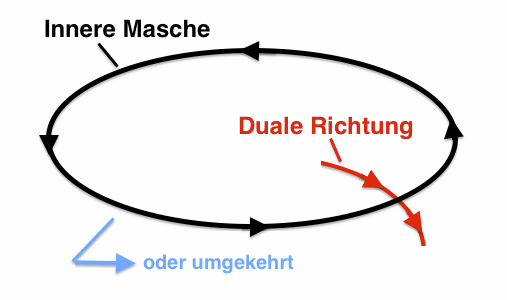
\includegraphics[width = 2.5cm]{./bilder/Duale_Richtung}}
	\item Dualfaktor $D [\Omega]$ wählen und Werte der dualen Netzwerk-Elemente
	bestimmen.
	
\end{enumerate}

\begin{multicols}{2}
\subsection{Netzwerkfunktionen}
\subsubsection{Grundformen}
	\begin{itemize}
		\item \textbf{Summenform:}\\
		 $\underline{F}(p) = K_0 \frac{p^n + a_1 p^{n-1} + \ldots + a_{n-1}p + a_n}{p^m+b_1 p^{m-1} + \ldots +b_{m-1}p+b_m} = K_0\frac{P_n(p)}{Q_m(p)}$
		\item \textbf{Produktform:}\\
		 $ \underline{F}(p) = K_0 \frac{(p-z_1)(p-z_2)\ldots(p-z_n)}{(p-p_1)(p-p_2)\ldots(p-p_m)}= K_0\frac{P_n(p)}{Q_m(p)}$
		\item \textbf{Normierte Produktform:}\\ \parbox{8cm}{Ausser konstantem Faktor $K$ nur Faktoren der Form: $p, (1+ap),(1+bp+cp^2)$ in Zähler und/oder Nenner!}
	%	\item \textbf{Partialbruchform:} Zu aufwändig?
	\end{itemize}
	\columnbreak
\subsection{Stabilitätsbedingungen}
\begin{tabular}{ll}
	stabil & alle Polstellen in der linken Halbebene\\
	grenzstabil & alle Polstellen in LHE und/oder auf
	$j\omega$-Achse\\
	instabil & mindestens eine Polstelle in der rechten Halbebene
\end{tabular}\\


\subsection{UTF zu Frequenzgang}
	$\underline{F}(p) \Rightarrow \underline{F}(jw)$
	$\rightarrow p$ mit $j\omega$ ersetzten!\\
	Multiplikation von konj. komplexen Polen:\\ 
		\hspace*{0.5cm}$(j\omega-(\sigma_1 + j\omega_1))(j\omega-(\sigma_1 - j\omega_1))$ \\ \hspace*{0.5cm}$= ((j\omega)^2-2j\omega\sigma_1+\sigma_1^2 +\omega_1^2)$
\end{multicols}

\subsection{Zusammenhang Polstellen - freie Schwingung}
\begin{multicols}{2}
\subsubsection{Allgemein}
\begin{itemize}
	\item \textbf{Term der freien Schwingung:}\\
		  $u(t)=c_1 e^{p_1 \cdot t}+c_2 e^{p_2\cdot t}+\ldots+c_m e^{p_m \cdot t}\quad
		  p_i$: Pole		
	 	\item \textbf{reeler Pol:} $\Rightarrow c_i\cdot 	e^{\sigma_i\cdot t} \rightarrow$ Pol bei $\sigma_i$
		\item \textbf{zweifach reeler Pol:}\\ $\Rightarrow c_i\cdot e^{\sigma_i\cdot t} + d_i \cdot t \cdot e^{\sigma_i\cdot t} \rightarrow$ zweifach Pol bei $\sigma_i$
		\item \textbf{konj. komplexer Pol:}\\
		$\Rightarrow \underline{c}_{i1}\cdot e^{(\sigma_i+j\omega_i)t} + \underline{c}_{i2}\cdot e^{(\sigma_i-j\omega_i)t} = A \cdot e^{\sigma_i t} \cdot cos(\omega_i\cdot t + \varphi)$ \\$\rightarrow$ Polstellen bei $\sigma_i \pm j\omega_i$
		
\end{itemize}

\subsubsection{Beispiel}
$u(t)=$\\$20Ve^{\frac{-t}{50ms}}-15V\cos(10s^{-1}t+\varphi_{11})+12Ve^{4s^{-1}t}\sin(5s^{-1}t+\varphi_{12})$\\ \\
Polstellen bei:
\begin{align}
	20Ve^{\frac{-t}{50ms}} = 20Ve^{-20s^{-1}t} &\rightarrow \text{Pol bei }
	-20s^{-1}\nonumber\\
	-15V\cos(10s^{-1}t+\varphi_{11}) &\rightarrow \text{Pol bei }
	(0\pm j10)s^{-1}\nonumber\\
	12Ve^{4s^{-1}t}\sin(5s^{-1}t+\varphi_{12}) &\rightarrow \text{Pol bei } (4\pm
	j5)s^{-1}\nonumber
\end{align}

%\begin{tikzpicture}[thick]
	\draw [->] (-3,0) -- (3,0);
	\node at (3,0) [anchor=west] {$\sigma$};
	\draw [->] (0,-3) -- (0,3);
	\node at (0,3) [anchor=south] {$j\omega$};
	\draw [dashed] (0,1) -- (1,1) -- (1,-1) -- (0,-1);
	\draw (-2.5,0) node[shape aspect=1,cross out,draw] {};
	\node at (-2.5,0) [anchor=north] {$-20s^{-1}$};
	\draw (0,2) node[shape aspect=1,cross out,draw] {};
	\node at (0,2) [anchor=west] {$j1000s^{-1}$};
	\draw (1,1) node[shape aspect=1,cross out,draw] {};
	\node at (1,1) [anchor=west] {$j500s^{-1}$};
	\draw (1,-1) node[shape aspect=1,cross out,draw] {};
	\node at (1,-1) [anchor=west] {$-j500s^{-1}$};
	\draw (0,-2) node[shape aspect=1,cross out,draw] {};
	\node at (0,-2) [anchor=west] {$-j1000s^{-1}$};
	\draw [->] (1.5,-0.5) -- (1.1,-0.1);
	\node at (1.5,-0.5) [anchor=west] {$4s^{-1}$};
\end{tikzpicture}\newline
\end{multicols}


\subsection{Zusammenhang PN-Verteilung \& Frequenzgang}
	\begin{tabular}{cp{14cm}}
		\parbox[c][5cm]{5.3cm}{\begin{tikzpicture}[thick]
	\draw [->] (-2.5,0) -- (2.5,0);
	\node at (2.5,0) [anchor=west] {$\sigma$};
	\draw [->] (0,-2) -- (0,2);
	\node at (0,2) [anchor=south] {$j\omega$};
	\draw [dashed] (-1,1) -- (1,1) -- (1,-1) -- (-1,-1) -- (-1,1);

	\draw (-2,0) node[shape aspect=1,cross out,draw] {};
	\draw (-1,1) node[shape aspect=1,cross out,draw] {};
	\draw (-1,-1) node[shape aspect=1,cross out,draw] {};
	
	\draw (1,-1) node[shape aspect=1,circle ,draw] {};
	\draw (1,1) node[shape aspect=1,circle ,draw] {};
	\draw (2,0) node[shape aspect=1,circle ,draw] {};

	\node at (-2,0) [anchor=north] {$-\sigma_2$};
	\node at (-1,0) [anchor=north] {$-\sigma_1$};
	\node at (1,0) [anchor=north] {$\sigma_1$};
	\node at (2,0) [anchor=north] {$\sigma_2$};
	
	\node at (0,1) [anchor=north west] {$j\omega$};
	\node at (0,-1) [anchor=north west] {$-j\omega$};
\end{tikzpicture}}
		& \parbox{14cm}
		  {\textbf{Frequenzgang:}\\ 	
			$\underline{F}(p) = K \cdot \frac{p-z_1}{(p-p_1)(p-p_2)} \Rightarrow \underline{F}(j\omega) = K\cdot \frac{jw-z_1}{(jw-p_1)(jw-p_2)} = K\cdot \frac{jw-\sigma_2}{(jw+\sigma_1-j\omega_1)(jw+\sigma_1+j\omega_1)}$\\
		  \textbf{Amplitudengang:}\\
		    $|\underline{F}(jw)| = K\cdot \frac{\overbrace{|j\omega-z_1|}^{A_{z_1}}}{\underbrace{|j\omega-p_1|}_{A_{p_1}}\underbrace{|j\omega-p_2|}_{A_{p_2}}}$
		    $ \Rightarrow$ \textbf{Allg.:} $\boxed{F(j\omega) = |K|\cdot\frac{\prod\limits^{n}_{i=1} A_{z_i}}{\prod\limits^{m}_{j=1} A_{p_j}}}$\\
		  \textbf{Phasengang:}\\
		  	\textbf{Allg.:} $\boxed{arg(\underline{F}(jw)) = \sum\limits_{i=1}^{n} \varphi_{z_i} - \sum\limits_{j=1}^{m} \varphi_{p_j} + k \pi}$\\
		  	Die Winkel liegen zwischen der Richtung der positiven $\sigma$-Achse und dem aktuellen $j\omega$.\\
		  	Eine Nullstelle auf der $j\omega$-Achse bewirkt einen Phasensprung von $\pi$.
		    }
\end{tabular}

%\subsection{DGL zu UTF}
%Ableitung wird zu $\cdot j \omega$:
%\[ \frac{du_2^2}{dt^2} + 3\frac{du_2}{dt} + u_2 = \frac{du_1}{dt} \longrightarrow (j\omega)^2u_2 + 3j\omega u_2 + u_2 = j\omega u_1
%\]

